\documentclass[12pt]{book}

\usepackage[ utf8x ]{ inputenc }
\usepackage[ romanian ]{ babel }

\usepackage{scrextend}

\usepackage[left=25mm, top=25mm,right=25mm]{geometry}

\usepackage{pdfpages}

\usepackage{graphicx}
\graphicspath{ {images/} }

\begin{document}
	
\title{Lucrare Licenta}
\maketitle
\tableofcontents
	
\chapter{Introducere}
\section{Motivare}
Tema lucrării mele de licență este denumită "Aplicație de gestionare a facturilor" și reprezintă dorința mea explicită de a face mai accesibil acest proces pentru toată lumea.

Plata electronică a facturilor este o caracteristică a mediului online și telefoniei bancare. Clientul unei instituții financiare transferă bani din contul său cu ajutorul cardului de credit către un creditor (utilitate publică, magazin, etc) sau către un alt individual. Aceste plăți sunt realizate, de obicei, electronic ca fiind un depozit direct prin intermediul sistemului național de plată, operate de bănci sau împreună cu guvernul. Adițional la plata facturilor, majoritatea băncilor oferă diferite caracteristici care vin odată cu sistemul electronic de plată al facturilor. Acestea includ abilitatea de a stabili plăți viitoare în avans la o dată respectivă, salvarea informațiilor companiei a cărei facturi s-a plătit și alte opțiuni de a căuta în istoria recentă a plăților. 

Deși această tehnologie a fost disponibilă pe la mijlocul anilor  '90, nu a fost foarte utilizată din cauza faptului că foarte puțină lume dispunea de internet. Începând cu anul 2000, plata electronică a facturilor a început să crească dramatic. 

Din punct de vedere al consumatorului, plata electronică a facturilor este mai ieftină, mai rapidă și mai agreată decât scrierea cecurilor sau completarea hârtiilor. Din punct de vedere al băncilor, această tehnologie a dus la scăderea semnificativă a consumui de hârtie și la creșterea fidelității clienților.

Totuși, în ciuda acestor progrese vizibile, procesul de plată a facturilor nu este foarte prietenos cu cei care sunt noi în domeniul tehnologiei și mai ales în domeniul internetului. Acesta este unul dintre motivele principale pentru care oamenii aleg să stea câte o ora la coadă decât să învețe să folosească internetul. Un exemplu de oameni din această categorie sunt părinții mei, care deși știu să utilizeze calculatorul, nu reușesc să plătească cu succes o factură în format electronic. 

Se spune că timpul este cea mai importantă bogăție a omului, deoarece odată pierdut nu mai poate fi recuperat. Și eu sunt de acord cu această afirmație și consider că  aplicația dezvoltată de mine reprezintă un mod foarte bun de a economisi timp. Cantitatea de timp nu este una foarte mare, dar în timp, această cantitate contează. Este mult mai ușor să plătești trei facturi în două minute decât să le plătești în zece minute sau chiar cincisprezece minute.

Viziunea mea pentru următorii 5 ani este aceea că majoritatea oamenilor vor plăti facturile prin intermediul internetului. Din acest motiv consider că domeniul plăților online va avea parte de îmbunătățiri continue și reprezintă o mare responsabilitate pentru mine faptul că am realizat cercetări în această arie.

Toate cele prezentate mai sus mi-au stârnit curiozitate și interesul si m-au determinat să aleg această temă pentru lucrarea mea de licență, iar acest lucru presupune să mă documentez cât mai serios cu privire la domeniul plăților online, să înțeleg cum funcționează toate aceste mecanisme și să caut o metoda de îmbunătățire a acestora din toate punctele de vedere. 

Lucrarea de licență este structurată în patru capitole.

Capitolul I conține partea de introducere în care se vorbește despre sursa de motivare care a stat în spatele cercetării și elaborării lucrării cât și a tehnologiilor care sunt deja în același domeniu.

Capitolul al II-lea prezintă tehnologiile folosite: Java, MySQL, Hibernate, PDFBox. Fiecare tehnologie este descrisă succint conținând și exemple din codul sursă al aplicației.

Capitolul al III-lea descrie funcționalitatea aplicației. Este descrisă fiecare operație în parte însoțită de imagini sugestive. 

Capitolul al IV-lea încheie lucrarea de licență prezentând care sunt planurile de viitor pentru dezvoltarea aplicației și care au fost dificultățile întâmpinate de-a lungul dezvoltării.
\section{Software existente}

Cel mai cunoscut software românesc în acest domeniu este platforma http://www.platifacturi.com. Aici utilizatorul își alege furnizorul (Orange, Telekom, Vodafone, RCS, UPC, E-ON, Enel sau distribuitorul local de apă pentru unele județe) după care va introduce numărul facturii, codul clientului și suma de plată. După completarea acestor câmpuri se verifică dacă datele introduse sunt corecte după care utilizatorului îi sunt cerute datele cardului (număr, data expirării, cod de securitate, deținătorul cardului). După ce utilizatorul a completat și aceste câmpuri se verifică validitatea lor după care se finalizează plata. Pentru fiecare factură plătită prin intermediul aceste platforme se percepe un comision de 0.95\% din totalul facturii, dar nu mai puțin de 1 LEU. 

O altă modalitate de a plăti electronic facturile este prin intermediul platformei companiei în cauză. De exemplu, fiecare abonat Orange deține sau poate să își creeze un cont de abonat și prin intermediul acestuia se pot plăti și vizualiza facturile. Această metodă este mai bună decât cea de mai sus deoarece nu se percepe niciun comision, un dezavantaj fiind faptul că dacă vrei să plătești factura Orange, Telekom, Enel, E-On ai nevoie de câte un cont de abonat la fiecare companie. 

\chapter{Tehnologii folosite}
\section{Java}
	
Java este un limbaj de programare orientat-obiect realizat de către James Gosling în cadrul companiei Sun Mycrosystems (acum filiala Oracle) și a fost creat să aibă cât mai puține dependențe legate de implementare. A fost creat ca să ajute dezvoltatorii de aplicații, limbajul fiind unul de tip WORA (Write Once Run Anywhere, traducere: Scrie odată rulează peste tot).  A fost lansat în anul 1995 iar de atunci a suferit o popularitate foarte mare, majoritatea aplicațiilor distribuite fiind scrise în Java, iar odată cu evoluția tehnologiei, limbajul de programare a devenit utilizat și la scrierea aplicațiilor mobile, agendelor telefonice, etc. Java este utilizat în prezent, având un real succes, și la programarea aplicațiilor destinate intranet-urilor. Astăzi, Java este unul dintre cele mai utilizate limbaje de programare, în special pentru aplicațiile web de tip client-server, având reportat un număr de 9 milioane de dezvoltatori.\cite{thinkJava}
	
Limbajul Java își însușește o mare parte din sintaxa limbajelor C și C++. Diferența dintre aceste limbaje este făcută în cadrul nivelului de jos al programării, Java având mai puține facilități, dar obiectul modelelor este de asemenea simplificat. Un program Java care este corect și care nu suferă modificări poate rula pe orice platformă care are instalată mașina virtuală Java(JVM care inseamnă Java Virtual Machine). Acest lucru este posibil deoarece codul scris în Java este compilat într-un format standard numit cod ce octeți( în engleză byte-code). Codul de octeți diferă față de codul mașină. Codul mașină poate fi executat fără a mai fi prelucrat deoarece este reprezentat de o secvență de instrucțiuni specifice unui anumit tip de procesor și a unei platforme binare de lucru. Codul de octeți reprezintă instrucțiuni asemănătoare codului scris in limbaj de asamblare. Compilatorul generează codul de octeți independent de platforma de lucru. Codul mașină este executat direct de către procesor și va putea rula numai pe platforma pe care a fost creat, pe când codul de octeți va putea rula pe orice platformă care are instalat mediul de programare Java deoarece codul de octeți este interpretat întocmai de acest mediu de programare. \cite{cursPracticJava}

Java Virtual Machine este disponibilă pentru toată lumea incepând din anul 2006, atunci când Sun a publicat un articol prin care anunțau că varianta companiei de JVM va fii open-source. Există și alți furnizori de JVM, printre care Oracle, IBM, Bea, FSF. \cite{thinkJava}

În funcție de modul de execuție a aplicaților, limbajele de programare se împart în două categorii:
\begin{addmargin}[4em]{1em}
	\begin{itemize}
		\item Interpretate: un program numit interpretor citește instrucțiunile linie cu linie și le traduce în instrucțiuni mașină. Această soluție prezintă un avantaj mare datorită simplității și a portabilității. Portabilitatea este dată de faptul că sursa programului este interpretată direct. Viteza de execuție redusă este un dezavantaj evident pentru această categorie. Limbajul de programare Basic este, probabil, cel mai cunoscut limbaj interpretat. 
		\item Compilate: compilatorul transformă codul sursă al programelor în cod care poate fi executat direct de către procesor. Acest cod se numește cod mașină. Un avantaj îl constituie execuția extrem de rapidă, de cealaltă parte, lipsa portabilității este un dezavantaj important. Un cod de nivel scăzut nu va putea rula decât pe platforma de lucru pe care s-a executat procesul de compilare. 
	\end{itemize}
\end{addmargin}
\bigbreak

Caracteristicile principale ale limbajului de programare Java au făcut ca acesta să fie, într-un interval relativ scurt, unul dintre cele mai populare și utilizate limbaje de programare. Caracteristicile principale ale limbajului sunt:
\begin{addmargin}[4em]{1em}
	\begin{itemize}
		\item Simplitate - supraîncărcarea operatorilor este eliminată, la fel și moștenirea multiplă și toate facilitățile care ar putea duce la scrierea unui cod confuz
		\item Ușurința cu care sunt create aplicațiile complexe (interfața grafică, firele de execuție, baze de date,etc).
		\item Robustețe - Renunțarea la pointeri duce la eliminarea unei surse foarte importante de erori, la fel și gestionarea automată a memoriei și eliminarea scurgerilor de memorie prin introducerea unei proceduri de colectare a obiectelor care nu mai sunt referite, procedura este numită "Garbage Collector".
		\item	Orientare pe obiecte completă - programarea procedurală este eliminată complet.
		\item Securitate - limbajul Java este unul foarte sigur deoarece furnizează mecanisme stricte de securitate (codul care verifică secvențele periculoase este verificat dinamic, atunci când se rulează procese la distanță sunt impuse niște reguli foarte stricte).
		\item Neutralitate arhitecturală - arhitectura fizică a mașinii pe care rulează aplicația nu influențează comportamentul acesteia.
		\item Portabilitate - independența față de platforma de lucru reprezintă un avantaj foarte mare pentru limbajul de programare și este o opțiune foarte bună pentru companiile dezvoltatoare de aplicații din cauza reducerii costurilor. Aplicațiile nu mai necesită recompilate și modificate la trecerea de la un sistem de operare la altul.
		\item	Este un cod compilat și interpretat, aceste două mari caracteristici definesc portabilitatea limbajului de programare.
		\item Performanță - recunoscut pentru faptul că limbajul este mai lent decât cele care generează executabile native pentru o anumită platformă de lucru, performanța ridicată a codului de octeți este asigurată de compilatorul Java, astfel încât viteza mai scăzută nu reprezintă un impediment dezvoltării aplicațiilor complexe ( animații, grafică 3D). \cite{cursPracticJava}
\end{itemize}
\end{addmargin}
\bigbreak	
Oracle a furnizat pentru Java 4 platforme:
\begin{addmargin}[4em]{1em}
\begin{itemize}
	\item Java Card – pentru smartcarduri (carduri cu cip)
	\item Java Platform, Micro Edition (Java ME) – pentru hardware cu resurse limitate gen telefoane mobile
	\item Java Platform, Standard Edition(Java SE)- pentru sisteme gen workstation ( gasim la PC-uri)
	\item Java Platform, Enterprise Edition(Java EE) – pentru sisteme de calcul mari \cite{thinkJava}
\end{itemize}
\end{addmargin}
\bigbreak
Mai multe versiuni au apărut de-a lungul timpului, și anume un număr de 9 versiuni. Acestea sunt :
\begin{addmargin}[4em]{1em}
\begin{itemize}
\item JDK 1.0 (1996) – versiunea inițială
\item JDK 1.1 (1997)
\item J2SE 1.2 (1998)
\item J2SE 1.3 (2000)
\item J2SE 1.4 (2002)
\item J2SE 5.0 (2004)
\item Java SE 6 (2006)
\item Java SE 7 (2012)
\item Java SE 8 (2014) 
\end{itemize}
\end{addmargin}
\bigbreak
Ultima versiune a limbajului Java (Java SE 8 -2014) este singura versiune gratis suportată de Oracle. \cite{cursPracticJava}
	
Un IDE (Integrated Development Environment) este, după cum spune numele, un mediu de lucru care permite dezvoltarea aplicațiilor specifice unui limbaj de programare. Pentru Java sunt următoarele : JCreator, Eclipse, NetBeans, BEA Workshop, BlueJ, CodeGuide, Dr Java, IntelliJ IDEA, JBuilder,JDeveloper, KDevelop.
	
Limbajul de programare Java a fost creat pe baza a cinci obiective majore:
\begin{addmargin}[4em]{1em}
\begin{enumerate}
	\item Trebuie să fie simplu, orientat pe obiect și familiar		
	\item Trebuie să fie robust și sigur.
	\item Trebuie să fie neutru din punct de vedere al arhitecturii și în același timp, portabil.
	\item Trebuie să fie executat cu performanță ridicată.
	\item Trebuie să fie interpretat, filetat și dinamic. 
\end{enumerate}
\end{addmargin}
\bigbreak
Oracle Corporation este proprietarul actual al implementării oficiale a platformei Java Standard Edition, ca urmare a achiziției companiei Sun Microsystems în anul 2010. Implementarea actuală este bazată pe implementarea originală facută de cei de la Sun. Implementarea Oracle este disponibilă pentru Microsoft Windows (încă merge și pentru Windows XP), Mac OS X, Linux și Solaris. 
	
Implementarea Oracle este distribuită în două moduri:
\begin{addmargin}[4em]{1em}
\begin{itemize}
\item The Java Runtime Environment (JRE) - conține părțile din platforma JAVA SE necesare pentru a rula programe Java 
\item The Java Development Kit (JDK) - este destinat programatorilor și conține programele de dezvoltare precum compilatorul Java, Javadoc, Jar și un debugger.\cite{JavaWiki}	
\end{itemize}
\end{addmargin}
\bigbreak
OpenJDK este altă implementare din familia JAVA SE care este sub licența GNU GPL. Implementarea a început când Sun a lansat codul sursă pentru Java sub licența GPL. Ca și în JAVA SE 7, OpenJDK este referința oficială a implementării limbajului de programare Java.

Scopul limbajului de programare Java este de a face compatibile toate implementările. De-a lungul istoriei, marca înregistrată a limbajului Java pentru utilizare (Sun trademark) a insistat ca toate implementările să fie compatibile. Acest lucru a iscat un conflict legal cu Microsoft după ce Sun a susținut că implementarea realizată de cei de la Microsoft nu avea suport pentru RMI (Remote Method Invocation) sau JNI (Java Native Interface) și au adăugat unele caracteristici specifice doar platformei lor. Sun a dat în judecată Microsoft în anul 1997, iar în anul 2001 au câștigat daune în valoare de 20 de milioane de dolari. Microsoft a fost de asemenea obligată să respecte termenii licenței impuși de Sun. Microsoft nu a acceptat acest lucru și începând din anul 2001 ei nu mai livrează Java împreună cu sistemul de operare Windows.

Platforma independentă Java este esențială către Java EE (Enterprise Edition) și este necesară o validare mai strictă  pentru a obține o implementare. Acest mediu permite aplicații portabile pe partea de server.

Programele scrise in limbajul Java sunt recunoscute pentru viteza scăzută și consumul mai mare de memorie față de cele scrise în limbajul C++. În orice caz, viteza de execuție a programelor scrise în Java s-a îmbunătățit semnificativ cu introducerea compilării “chiar la timp” în anul 1997/1998 pentru versiunea Java 1.1, adăugarea de noi caracteristici pentru limbaj suportă o mai bună analiză a codului (clase în clase, clasa StringBuilder, optimizări în mașina virtuală Java). Odată cu versiunea 1.5, performanța a fost îmbunătățită cu adăugarea pachetului java.util.concurrent. Această implementare a fost îmbunătățită ulterior cu versiunea 1.6.

Unele platforme oferă suport hardware direct pentru Java, există microcontrollere care rulează Java în hardware și nu în mașina virtuală, și procesoare ARM care oferă suport pentru execuția codului de octeți Java.

Java utilizează un Garbage Collector automat pentru organizarea memoriei în ciclul de viață al unui obiect. Programatorul determină când sunt create obiectele iar Java runtime este responsabil cu recuperarea memoriei odată ce obiectele nu mai sunt utilizate. Odată ce nu rămân referințe la obiecte, memoria neaccesibilă devine disponibilă pentru eliberare automată de către Garbage Collector. Ceva similar unei scurgeri de memorie poate să apară dacă codul implementat de programator stochează o referință la un obiect care nu mai este nevoie de el, de obicei apare acest lucru când obiectele de care nu mai sunt nevoie sunt stocate în containere care încă sunt utilizate. Dacă sunt executate operații asupra unui obiect neexistent, va fi aruncată excepția “Null Pointer Exception”. 

Una din ideile din spatele organizării automate a memoriei este aceea că programatorii sunt scutiți de povara de a face manual administrarea memoriei. În unele limbaje de programare, memoria pentru creare obiectelor este alocată implicit în stack (grămadă), sau explicit alocată și dealocată în memoria heap, în acest ultim caz, programatorului îi revine responsabilitatea de a administra memoria. Dacă programul nu dealocă obiectul, va apărea o scurgere de memorie. Dacă programul încearcă să acceseze sau dealoce o zonă de memorie care a fost deja dealocată, rezultatul nu este definit și este dificil de prezis, iar programul este foarte probabil să devină instabil sau să se distrugă. Acest lucru poate fii remediat parțial utilizând pointeri smart, dar aceștia adaugă o complexitate mai mare. De reținut este faptul că Garbage Collector-ul nu previne scurgerile de memorie, acele cazuri în care memoria este referențiată dar nu este folosită.

Procesul de colectare a resturilor poate să aibă loc în orice moment. De obicei, va porni atunci când un program este inactiv. Este garantat că procesul va fi declanșat daca nu mai este suficientă memorie heap liberă pentru a crea un nou obiect. Acest lucru poate duce la o pauză a procesului de rulare a programului pentru un moment. Administrarea explicită a memoriei nu este posibilă in Java.\cite{thinkJava}

Java nu suportă operațiile aritmetice cu pointeri din C sau C++, unde adresele obiectelor și valorile de tip usigned int (sau long int) pot fi utilizate pentru interschimbare. Acest lucru alocă colectorului de deșeuri (garbage collector) să realoce obiectele referențiate și să asigure securitatea și siguranța .

Ca și în C++ sau în alte limbaje de programare orientată obiect, variabilele tipurilor primitive de date din Java sunt stocate direct in câmpuri (pentru obiecte) sau în stack (pentru metode) și nu în zona de memorie heap. Această decizie a fost luată de designerii Java din motive de performanță.

Limbajul de programare Java conține diferite tipuri de colectoare de deșeuri (garbage collectors). În mod implicit, HotSpot foloseste “parallel scavenge garbage collector”. În orice caz, sunt multe alte colectoare de deșeuri care pot fi utilizate pentru administrarea memoriei heap. Pentru 90\%  din aplicațiile Java, este suficient utilizarea colectorului de deșeuri “Concurrent Mark-Sweep (CMS)”. Oracle tinde să înlocuiască colectorul de deșeuri CMS cu colectorul “Garbage First Collector (G1) “.\cite{thinkJava}

Limbajul de programare Java folosește, în mod nativ, setul de caractere Unicode. Acesta este un standard internațional care a dus la înlocuirea codului ASCII ( vechiul set de caractere). In setul Unicode, caracterele sunt reprezentate cu ajutorul a 2 octeți ( față de codul ASCII unde se pot reprezentate numai 256 de caractere, setul Unicode suportă reprezentarea a unui număr maxim de 65536 de caractere). Primele 256 de caractere din setul Unicode sunt la fel ca și cele din codul ASCII. Pentru referirea celorlalte caractere se folosește sintaxa \%uxxxx, unde xxxx reprezintă codul caracterului. O caracteristică importantă a setului de date Unicode o reprezintă și faptul că întreg intervalul de reprezentare a simbolurilor este împărțit în subintervale, purtând denumirea de blocuri. Exemple de blocuri: Basic Latin, Gothic, Greek, Arabic, Arrows, Currency, Mathematical, Musical, etc. \cite{cursPracticJava}

Abstract Window Toolkit (AWT) este o parte Java care se ocupă cu crearea interfețelor grafice și desenarea graficelor și a imaginilor. Este un set de clase create cu scopul de a pune la dispoziția programatorului tot ce are nevoie pentru a crea o interfață grafică pentru o aplicație Java. Majoritatea componentelor AWT sunt derivate din clasa de bază java.awt.Component. Acest lucru este ilustrat în figura de mai jos:
\begin{center}
	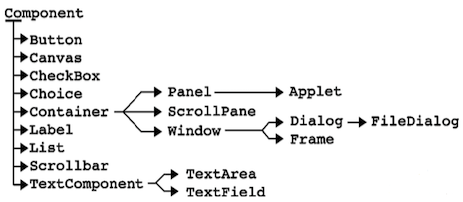
\includegraphics{awt}
	\cite{swingBook}
\end{center}

Java Foundation Classes (JFC) este alcătuită din cinci părți majore: AWT, Swing, Accesibility, Java 2D și Drag and Drop. Java 2D a devenit o parte integrală a AWT, Swing este construit pe baza AWT iar Accesibility este contruit în Swing. Cele cinci părți ale JFC nu sunt exclusiv independente, este de așteptat ca Swing să se muleze și mai mult cu AWT în versiunile viitoare. Prin urmare, AWT este nucleul JFC, ceea ce o face una dintre cele mai importante librării în Java 2.

Swing este un set mare de componente începând de la etichete și până la tabele, arbori și documente complexe. Aproape toate componentele Swing sunt derivate de la o singură clasă, și anume JComponent. JComponent extinde clasa AWT Cointainer. Din acest motiv, Swing este cel mai bine descris ca fiind un strat care stă deasupra componentei AWT și nu un strat care o înlocuiește. Fiecare component AWT are un echivalent în Swing care începe cu prefixul "J". Singura excepție de la această regulă o face clasa AWT Canvas. Ca echivalent al acestei clase, se folosește JLabel, JPanel sau JComponent. De asemenea, există și clase Swing care nu au un reprezentant în AWT. Figura de mai jos reprezintă o mică parte din librăria Swing, dar această parte conține clasele cu care programatorii se confruntă cel mai mult. Celelalate clase Swing oferă suport și customizare pentru clasele aceastea:
\begin{center}
	\includegraphics{swing}
	\cite{swingBook}
\end{center}
\section{MySQL}
Un sistem de organizare a unei baze de date relaționale este o implementare necesară în foarte multe domenii, de la lucruri tradiționale la afaceri, cercetări, contexte educaționale, la aplicații foarte puternice și complexe ( de exemplu, motoarele de căutare pe internet). În ciuda faptului că o bază de date este foarte importantă pentru a administra și accesa resursele informative, multe organizații s-au aflat în imposibilitatea financiară de a avea un asemenea sistem. De-a lungul timpului, sistemele de baze de date au fost o propunere destul de scumpă, furnizorii cerând sume importante de bani atât pentru partea de software cât și pentru partea de suport. Deoarece un sistem de baze de date necesită echipament hardware substanțial pentru a rula cu o performanță decentă, costul total a devenit și mai mare. 

Situația este diferită în zilele noastre, atât din punct de vedere software cât și hardware. Sistemele micuțe desktop și serverele sunt ieftine și eficiente și este o dorință arzătoare a companiilor dezvoltatoare să scrie sisteme de operare cât mai rapide pentru aceste instrumente. Aceste sisteme de operare sunt distribuite în mod gratuit pe internet. Ele includ și câteva derivate Unix BSD (FreeBSD, NetBSD, OpenBSD) la fel și multe distribuții ale sistemului de operare Linux (Fedora, Debian, Gentoo, Suse și multe altele). \cite{mySqlDeveloperLibrary}

Producția de sisteme de operare gratuite a început odată cu dezvoltarea aplicațiilor gratuite ca și GCC, compilatorul GNU C. Aceste eforturi de a face software-ul disponibil oricui are nevoie de el fac parte din mișcarea Open Source. Proiectele Open Source au produs lucruri importante în industria software. De exemplu, Apache este cel mai utilizat server web pe internet. Perl, Python și Ruby sunt limbaje de scripting foarte utilizate și totodata foarte stabile, iar PHP este un limbaj care a devenit popular din cauza ușurinței cu care se pot scrie pagini web dinamice. Toate aceste lucruri sunt în contrast cu soluțiile aflate în proprietatea cuiva și au un preț foarte ridicat și nici măcar nu există acces la codul sursă al acestor programe.

Software-ul pentru bazele de date a devenit și el mai accesibil iar sistemele Open Source de administrare a bazei de date sunt disponibile gratuit. Unul dintre acestea este MySQL, un sistem SQL de tip client-server utilizat la administrarea bazei de date relaționale și este originar din Scandinavia. MySQL include un server SQL, programe care să permită clientului să acceseze serverul SQL, programe administrative și interfețe pentru a scrie propriile programe.\cite{mySqlDeveloperLibrary}

Rădăcinile MySQL au prins naștere în anul 1979, când Michael Monty Widenius de la compania suedeză TcX a creat o aplicație pentru baze de date numită UNIREG. În anul 1994, compania TcX a început să caute un sistem de administrare a bazei de date relaționale cu o interfață SQL pentru a putea fi folosită în dezvoltarea aplicațiilor web. Au testat câteva servere comerciale, dar au descoperit doar faptul că erau prea lente  pentru tabelele foarte largi ale companiei. De asemenea, au investigat și programul mSQL, dar acesta nu dispunea de multe proprietăți pe care compania TcX le-a marcat ca fiind necesare. 

Prin urmare, Monty a început dezvoltarea unui nou sever. Interfața de programare a fost creată explicit să fie similară cu cea folosită de aplicația mSQL deoarece multe aplicații gratuite erau disponibile pentru mSQL, și folosind o interfață similară, toate acele aplicații gratuite puteau fii folosite și pentru MySQL cu un minimum efort de portabilitate. 

În anul 1995, David Axmark de la compania Detron HB a început să îi stimuleze pe cei de la TcX să lanseze MySQL pe internet. David a lucrat, de asemenea, și la documentație și la posibilitatea ca MySQL să ruleze cu utilitățile GNU. MySQL 3.11.1 a fost lansat în toată lumea în anul 1996 sub forma unor distribuții binare pentru sistemele de operare Linus și Solaris. Astăzi, MySQL este disponibil în mult mai multe platforme atât sub formă binară cât și sub formă de cod sursă. Compania MySQL AB a fost formată pentru a pune la dispoziție distribuții MySQL atât pentru versiunea Open Source cât și pentru cele cu licență comercială și să ofere suport tehnic, servicii de monitorizare și training. În anul 2008, compania Sun Microsystemsa achiziționat compania MySQL AB ( angajamentul pentru versiunea Open Source a continuat să fie la fel de puternic deoarce planul companiei Sun era de a distribui majoritatea produselor lor sub forma Open Source).

Inițial, MySQL a devenit popular la scară globală pentru viteza și simplitatea sa. MySQL nu a fost lipsit de critici, mai ales din cauza faptului că îi lipsea multe caracteristici printre care tranzacțiile și suport pentru cheia străină. MySQL a continuat să se dezvolte adăugând nu doar acele caracteristici lipsă cât și altele, printre care amintim replicațiile, subinterogările, procedurile stocate, vederi și trigerr-e (declanșatoare). Aceste capabilități au dus MySQL pe tărâmul aplicațiilor enterprise (aplicații care sunt destinate mai degrabă companiilor și nu utilizatorilor individuali). Ca și rezultat, oamenii care odată considerau aplicațiile de tip "big iron" (calculatoare foarte mari, foarte rapide dar și foarte scumpe) potrivite pentru implementarea unui sistem de baze de date, acum acordă foarte mare atenție MySQL. 

MySQL este portabil și rulează pe sistemele de operare comerciale (cum ar fi Mac OS X, Windows, HP-UX) și pe dispozitive hardware până la rangul de sus, reprezentat de serverele companiilor foarte mari. Mai mult decât atât, performanța sa concurează cu peformanța oricărui sistem de baze de date și poate să găzduiască baze de date care conțin miliarde de rânduri. În domeniu afacerilor, MySQL continuă să își mărească prezența deoarece companiile descoperă că MySQL poate fi capabil să le gestioneze baza de date la o zecime de preț față de cât plăteau de obicei pentru licențele comerciale și suport.

MySQL face parte din categoria sistemelor de operare gratis care rulează pe compenente hardware foarte puternice dar ieftine, punând puterea substanțială de procesare și capabilitățile în mâinile unor utilizatori individuali și ale unor afaceri, mai mult ca oricând, pe o varietate foarte largă de sisteme. Această coborâre a barierelor economice în domeniul calculatoarelor a făcut ca soluțiile foarte rapide de baze de date să ajungă la mai mulți oameni și la mai multe organizații decăt oricând altcândva. Organizațiile care doar visau să aibă un sisteme de administrare a unei baze de date relaționale, pot face acest lucru la un cost foarte scăzut. Acest lucru este adevărat și pentru utilizatori individuali.

Multe sisteme de administrare a bazei de date sunt disponibile gratuit sau la un cost foarte mic, printre care MySQL, PostgreSQL sau SQLite. Atunci când comparăm MySQL cu alte sisteme de acest tip trebuie să ne gândim la cele mai importante lucruri: performanță, suport, caracteristici disponibile, condiționare și restricționare a licenței și preț. Luând toate acestea în considerare, MySQL are foarte multe lucruri atrăgătoare de oferit:
\begin{addmargin}[4em]{1em}
\begin{itemize}
	\item Viteza. MySQL este foarte rapid. Dezvoltatorii acestui sistem susțin că este cel mai rapid sistem de administrare a bazei de date relaționale. 
	\item Ușor de utilizat. MySQL este foarte performant dar relativ simplu și este mult mai puțin complex de setat și administrat decât sistemele mai mari.
	\item Suport pentru interogări. MySQL întelege limbajul SQL (Structured Query Language), limbajul standard pentru sistemele de baze de date moderne.
	\item Capabilitate. Serverul MySQL este multi-thread (mai mult fire de execuție) ața că mai mulți clienți pot să pot să se conecteze la el în același timp. Fiecare client poate să folosească mai multe baze de date în același timp. Accesarea serverului se poate realiza interactiv folosind diferite interfețe care permit adăugarea de interogări și vizualizarea de operații: clienți din linia de comandă, browser-e web sau aplicații grafice. În completare, interfețe de programare sunt disponibile pentru multe limbaje, de exemplu: C, Perl, Java, PHP, Python și Ruby. Putem să accesăm MySQL și cu ajutorul aplicațiilor care suportă ODBC și .NET (protocoale dezvoltate de Microsoft). Acest lucru ne dă posibilitatea de a scrie prepachetele noastre pentru client în vederea accesării informațiilor din baza de date.
	\item Conectivitate si securitate. MySQL este complet de tip rețea iar bazele de date pot fi accesate de oriunde există conexiune la internet, deci poți să împărtășești datele cu oricine, oriunde. Dar, în același timp, MySQL controlează accesul la informație așa încât o persoană care nu are dreptul de a vizualiza conținutul bazei de date nu va putea face acest lucru. Ca să ofere securitate și mai mare, MySQL suportă conexiuni criptate folosind protocolul SSL (Secure Sockets Layer).
	\item Portabilitate. MySQL rulează pe o varietate foarte mare de sisteme de operare de tip Unix și Linux, la fel și pe alte sisteme cum ar fii Windows și NetWare. MySQL rulează pe echipamente hardware de la servere foarte mari până la dispozitive care încap în palmă. 
	\item Spațiu redus. MySQL este distribuit pe o dimensiune redusă, mai ales comparativ cu uriașele discuri de stocare ale altor sisteme de baze de date.
	\item Disponibilitate și cost. MySQL este un proiect disponibil de tip Open Source sub mai multe licențe. În primul rând, este disponibil sub licența celor de la GNU General Public License (GPL). Acest lucru însemnând că MySQL este disponibil fără niciun cost pentru majoritatea operațiilor necesare. În al doilea rând, organizațiile care preferă aranjamentele formale sau nu vor să fie legate de condițiile de licențiere a celor de la GPL, licențele comerciale sunt disponibile.
	\item Distribuție deschisă și codul sursă. MySQL este foarte ușor de obținut. Trebuie doar să folosești browserul web. Dacă nu înțelegem cum funcționează o caracteristică sau vrem să facem un audit de securitate, putem să obținem codul sursă și să îl examinăm. Dacă utilizatorul care inspectează codul sursă găsește ceva in neregulă, este recomandat să raporteze această eroare pentru a putea fi corectată.\cite{mySqlDeveloperLibrary}
\end{itemize}
\end{addmargin}
\bigbreak
Distribuția MySQL include următoarele unelte:
\begin{addmargin}[4em]{1em}
\begin{itemize}
\item Un server SQL. Acesta este motorul care pornește MySQL și oferă acces la baza de date.
\item Programul pentru client și pentru alte utilizări. Acestea includ un program interactiv pentru client care permite acestuia să introducă direct interogările și să vizualizeze rezultatele. De asemenea sunt disponibile mai multe programe administrative care te ajută să rulezi MySQL împreună cu site-ul tău: un program permite administratorului să monitorizeze și să controleze serverul, alte programe permit acestuia să importe date, să își salveze datele la un interval de timp (proces numit back-up), să verifice tabelele de probleme și multe alte chestii.
\item O librărie pentru client care să îi permită să scrie propriile programe. Se pot scrie programe client în limbajul C deoarece librăria este creată în C. Librăria poate fi corelată cu alte limbaje de programare precum Perl, PHP, Ruby pentru a oferi serviciile de bază pentru intefețele MySQL.\cite{mySqlDeveloperLibrary}
\end{itemize}
\end{addmargin}
\bigbreak
Adițional software-ului disponibil împreună cu MySQL, MySQL este utilizat de mulți oameni talentați și capabili cărora le place să scrie software pentru a-și mări productivitatea și care sunt disponibili să împărtășească acest program. Rezultatul este unul benefic, accesul la o varietate largă de unele care fac MySQL să fie mai ușor de utilizat sau de integrat în diferite arii, cum ar fi dezvoltarea de site-uri web. \cite{mySqlDeveloperLibrary}

\section{Hibernate}
Majoritatea proiectelor de dezvoltare software implică cel puțin o bază de date relațională. Baza majorității aplicațiilor comerciale este reprezentată de informație ordonată la scară mare, de exemplu: cataloage, liste de clienți, detalii de contracte, texte plublicate sau design arhitectural.

Odată cu apariția World Wide Web ( rețea largă internațională), cererea pentru baze de date a crescut considerabil. Chiar dacă poate nu știu, clienții unei librării online, de exemplu, sau a unui ziar online necesită folosirea unei baze de date pentru stocarea lor. Undeva în adâncul aplicației, o bază de date este interogată și un răspuns al acesteia este oferit. 

Hibernate este o arhitectură care simplifică utilizarea bazelor de date relaționale în aplicațiile realizate cu ajutorul limbajului de programare Java. Acest lucru este posibil reprezentând datele relaționale ca fiind simple obiecte, accesate în urma unei sesiuni. Hibernate prezintă două tipuri de interfete programabile: o interfață nativă Hibernate și The Java EE-standard Java Persistence API. 

Sunt situații în care utilizarea Hibernate este foarte utilă, dar sunt și situații pentru care abordarea tradițională reprezentată prin accesul direct via The Java Database Connectivity (JDBC) Api este recomandată. Totuși, Hibernate rămâne favorită pentru prima opțiune deoarece nu exclude nici folosirea simultană a mai multor abordări, deși trebuie avută foarte mare grijă atunci când datele sunt modificate cu ajutorul a două API-uri diferite.

Hibernate nu a fost creat pentru a rezolva o problemă ci deoarece atunci când facem exact aceleași lucruri folosing JDBC, avem nevoie de o cantitate considerabilă de cod și de observarea atentă a diferitelor reguli (de exemplu, administrarea conexiunilor) ca să ne asigurăm că aplicațiia noastră nu produce o scurgere de resurse. 

	

Într-o lume ideală ar fi neimportant să luăm orice obiect Java și să îl persistăm într-o bază de date. Nicio introducere de cod nou nu va fi necesară pentru a realiza această caracteristică, nu vor apărea nici penalități de performanță iar rezultatul va fi portabil în totalitate. În această lume ideală probabil că vom realiza operația respectivă în următorul mod:\\
POJO pojo = new POJO();\\
ORMSolution magic = ORMSolution.getInstance();\\
magic.save(pojo);\\
Nu vor apărea surprize neplăcute, nu va fi nevoie de muncă în plus pentru a corela clasele cu tabelele bazei de date iar performanța nu va afectată.\cite{BeginningHibernate}

Hibernate este foarte aproape de această lume ideală, cel puțin atunci când este comparată cu celelalte alternative, dar este nevoie de crearea unor fișiere de configurare și trebuie luate în calcul și problemele de performanță și sincronizare. Hibernate, în orice caz, își atinge scopul fundamental: permiterea stocării de obiecte de tip POJO (Plain Old Java Object) în baza de date. 

Termenul comun pentru persistența directă a obiectelor Java este "obiect/ mapare relațională", care înseamnă maparea obiectelor Java direct la entitățile relaționale ale unei baze de date. Următoarea imagine arată modul în care Hibernate se mulează într-o aplicație, de la codul clientului și până la baza de date:
\begin{center}
	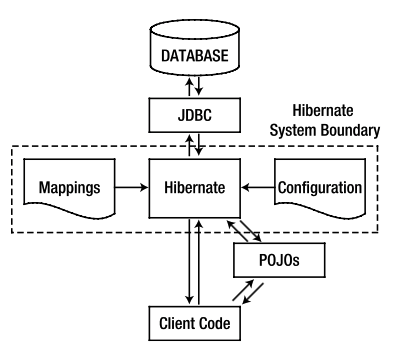
\includegraphics{Hibernate}
\end{center}
\cite{BeginningHibernate}
Comparativ cu JDBC, Hibernate furnizează o administrare a resurselor mai curată, acest lucru însemnând faptul că nu mai trebuie să ne îngrijorăm de conexiunile actuale ale bazei de date sau de a introduce blocuri gigantice de cod de tipul "try/catch/finally".
Totuși, erorile nu vor dispărea, doar că nu va mai trebui să ne ocupăm noi de ele. În orice caz, aceste condiții sunt excepționale (adică ne ocupăm doar de excepțiile de care trebuie să ne ocupăm, nu de fiecare excepție care ar necesita tratament).

Hibernate manipulează maparea obiectelor la tabelul bazei de date incluzând construirea schemei bazei de date dacă o configurăm să facă acest lucru. Nu necesită construirea unui tabel pentru fiecare tip de obiect, putem să mapăm foarte ușor un obiect la mai multe tabele. Și, de asemenea, Hibernate administrează și relațiile dintre obiecte, de exemplu: dacă am adăugat o listă de adrese unei persoane, putem foate ușor să avem adresele stocate intr-un al doilea tabel, construit și organizat de Hibernate.

Pornirea Hibernate durează puțin mai mult decât codul direct JDBC. Oricum, timpul de inițializare a sistemului nu este o măsură foarte semnificativă. Majoritatea aplicațiilor au perioade foarte lungi de rulare iar procentul de timp petrecut în procesul de inițializare a librăriei Hibernate este nesemnificativ comparativ cu performanța actuală a aplicațiilor. Avantajele Hibernate în întreținerea și administrarea obiectelor mai mult decât compensează timpul utilizat în configurare și inițializare. Ca de obicei, cel mai bun mod de a evolua performanțele unei aplicații este de a testa și a analiza aplicația propriu-zisă.

Orice obiect Java capabil de a fi persistat la o bază de date este un candidat pentru a fi persistat cu ajutorul Hibernate. Prin urmare, Hibernate este o înlocuire naturală pentru soluțiile ad-hoc (ca și JDBC de examplu) sau un motor de persistare pentru o aplicație care nu are deja încorporată o bază de date. În plus, prin alegerea Hibernate, utilizatorul nu este legat de nicio decizie (schimbarea designului, de exemplu) pentru obiectele aflate în aplicație, incluzând care bază de date să fie folosită pentru Hibernate.

După cum era de așteptat, Hibernate are nevoie de cineva să îi spună care tabel corespunde cărui obiect. În limbajul Hibernate, acest proces este numit mapare. Mapările pot fi implementate prin adnotări Java sau cu ajutorul unui fișier de mapare XML. Adnotările sunt preferate de majoritatea dezvoltatorilor deoarece oferă o imagine clară a structurii chiar la nivelul de cod. Hibernate dispune și de o abordare de tipul "configurare prin excepție" pentru adnotări: dacă suntem mulțumiți cu valorile pe care Hibernate ni le prezintă, nu mai trebuie să le precizăm explicit cu ajutorul adnotărilor. Pentru instanțe, Hibernate folosește numele clasei POJO ca și valoarea implicită a tabelului bazei de date pentru care se realizează maparea. De fapt, dacă accesul la baza de date se realizează doar prin intermediul Hibernate, nu trebuie să știm numele tabelului. Acest lucru este posibil deoarece interogările Hibernate se realizează pe tipul obiectului și nu pe numele tabelului. Hibernate construiește automat interogarea în așa fel încât este folosit numele corect al tabelului, chiar dacă ulterior schimbăm numele tabelului. \cite{BeginningHibernate}

Integrarea Hibernate în aplicația Java se realizează relativ ușor. Designer-ii Hibernate au evitat câteva dintre cele mai comune capcane și probleme care existau cu soluțiile persistenței Java și au creat o arhitectură curată și puternică în același timp. Practic, acest lucru înseamnă că nu e nevoie să rulăm Hibernate în interiorul unui container sau schelet Java EE. Rularea Hibernate necesită doar instalarea versiunii Java 6 sau versiuniile următoare.

La început, adăugarea Hibernate în proiectul Java poate să intimideze utilizatorul deoarece distribuția include un set foarte mare de librării. Pentru a avea prima aplicație Hibernate, trebuie setate referințele bazei de date și configurările Hibernate, care pot include maparea obiectelor la baza de date. De asemenea, trebuie creată și clasa de tip POJO împreună cu toate adnotările folosite în procesul de mapare. După ce au fost făcute toate acestea de mai sus, trebuie scrisă partea logică din spatele aplicației care utilizează Hibernate în vederea obținerii unor rezultate. Odată ce procesul de integrare Hibernate într-o aplicație Java este înțeles, chestiile de bază se aplică pentru orice proiect care folosește Hibernate.

Una dintre caracteristicile cheie a Hibernate este faptul că Hibernate nu interferează cu aplicația Java mai mult decât este nevoie, acest lucru a fost posibil datorită designer-ilor care au creat Hibernate. 

Pentru a configura și integra Hibernate este necesar parcurgerea următorilor pași:
\begin{addmargin}[4em]{1em}
	\begin{enumerate}
	\item Identificarea claselor de tip POJO care trebuie reprezentate cu ajutorul bazei de date.
	\item Indentificarea proprietăților clasei POJO care trebuie persistate (mapate)
	\item Adnotarea fiecărei proprietăți pentru a mapa obiectele Java la numele coloanelor bazei de date
	\item Crearea schemei bazei de date folosing unealta pentru exportarea schemei, folosind o bază de date actuală sau crearea propriei scheme a bazei de date.
	\item Adăugarea librăriilor Hibernate în aplicația Java.
	\item Crearea unui fișier XML de configurare Hibernate care indică spre baza de date și spre clasele mapate acesteia.
	\item În aplicația Java, trebuie creat un obiect de tip Hibernate Configuration care face referire la fișierul de configurare XML.
	\item Tot în aplicația Java, trebuie creat un obiect de tipul Hibernate SessionFactory din obiectul Configuration.
	\item Restabilește obiectele de tip HibernateSession din sesiunea FactorySession și scrie datele pentru accesul logic al aplicației ( crează, șterge, actualizează,etc).\cite{BeginningHibernate}
\end{enumerate}
\end{addmargin}

Utilizatorul poate chema Hibernate direct din aplicația Java sau poate accesa Hibernate prin intermediul unei alte arhitecturi. Putem chema Hibernate prin intermediul unei aplicații de tip Swing, unui servlet, portlet, unei pagini JSP sau prin intermediul oricărei aplicații Java care are acces la o bază de date. De obicei, Hibernate este utilizat pentru a crea un înveliș pentru accesul de date al aplicației sau pentru a înlocui un înveliș existent.

Hibernate suportă Java Management Extensions (JMX), J2EE Connector Architecture (JCA) și Java Naming and Directory Interface (JNDI). Folosing JMX, putem configura Hibernate în timp ce rulează. Hibernate poate fi lansat ca un conector de tip JCA și putem utiliza JNDI pentru a obține sesiunea curentă Hibernate. Adițional, Hibernate folosește driverele standard JDBC pentru a accesa baza de date relațională. Hibernate nu înlocuiește JDBC în vederea conectării și executării de operații asupra bazei de date. Hibernate se folosește de JDBC în executarea operațiilor respective.

Adițional standardului JAVA APIs, majoritatea aplicațiilor Java de tip web integrează Hibernate. API-urile simple și curate Hibernate fac integrarea Hibernate ușor de suportat într-un fel sau altul. Scheletul Spring distribuie un excelent mod de a integra Hibernate, incluzând suport generic pentru obiectele persistente, un set generic de excepții și o administrare a tranzacțiilor.

Neținând cont de mediul în care este integrat Hibernate, anumite cerințe rămân constante. Trebuie definite detaliile configurației care se aplică. Aceste detalii sunt reprezentate, în pasul următor, de un obiect de tip Configuration. De la acest obiect se crează un singur obiect de tipul SessionFactory. De la acest obiect, obiectele de tip Session sunt instanțiate, obiecte prin care aplicația accesează reprezentarea Hibernate a bazei de date. \cite{BeginningHibernate}

\section{Apache PDFBox}

Apache PDFBox este o librărie pentru limbajul de programare Java de tip Open Source care lucrează cu documentele de tip PDF. Permite crearea de documente noi de tip PDF, manipularea documentelor existente cât și abilitatea de a extrage conținutul documentelor. Apache PDFBox include, de asemenea, importante utilități pentru linia de comandă. Apache PDFBox este publicat sub licența Apache License v2.0.\cite{PDFBoxOfficial}

Apache PDFBox conține următoarele componente:
\begin{addmargin}[4em]{1em}
	\begin{itemize}
		\item PDFBox: partea de bază
		\item FontBox: se ocupă cu informațiile despre fonturi
		\item XmpBox: se ocupă de metadatele de tip XMP
		\item Prefligh (componentă opțională): verifică fișierele PDF în conformitate cu standardul PDF\%-1a \cite{PDFBoxOfficial}
\end{itemize}
\end{addmargin}

Dezvoltarea PDFBox a început în anul 2002 în cadrul companiei SourceForge de către Ben Litchfield care a vrut să extragă textul din fișierele PDF pentru librăria Lucene. A devenit parte a proiectului Apache Incubator în anul 2008 iar în anul 2009 a ajuns unul dintre proiectele de top ale companiei. În anul 2015, ApachePDFBox a fost numit partener a organizației Open Source Partner Organization de către PDF Association.

Una dintre caracteristicile importante a uneltei Apache PDFBox este aceea de a extrage rapid și precis text dintr-o varietate de documente de tip PDF. Această funcționalitate este încapsulată în org.apache.pdfbox.util.PDFTextStripper și poate fii executat foarte ușor din linia de comandă. 

Lucene este o librărie de căutare a textului de tip Open Source făcând parte din proiectul Apache Jakarta Project. Pentru ca Lucene să poată indexa un document PDF, trebuie prima dată să fie convertit sub formă de text. PDFBox dispune de o abordare simplă pentru a adăuga documentele PDF într-un index Lucene.\\
\\
Document luceneDocument = LucenePDFDocument.getDocument( ... );\\

După ce s-a creat obiectul de tip Lucene Document, poate fii adăugat la indexul Lucene în același mod ca și când ar fi fost creat dintr-un fișier text sau HTML. LucenePDFDocument extrage automat o varietate de câmpuri de metadate din fișierul PDF care sunt adăugate indexului Lucene, javadoc afișând detaliile în acele câmpuri. Această abordare este foarte simplă și este suficientă pentru majoritatea utilizatorilor, în caz contrar se pot utiliza tehnici mai avansate de extragere a textului.\cite{PDFBoxOfficial}

Unele aplicații conțin cerințe mai complexe de extragere a textului, nici linia de comandă sau LucenePDFDocument nu pot îndeplinească acele cerințe. Este posibil ca utilizatorul să utilizeze sau să extindă clasa PDFTextStripper pentru a satisface o parte din cerințele respective.

Există destule moduri de a limita textul care este extras în timpul procesului de extragere. Cel mai simplu mod este de a specifica intervalul de pagini din care să se extragă textul. 

Extragerea textului în limbile ale căror conținut merge de la dreapta la stânga  (Arabă sau Ebraică, de exemplu) poate să rezulte în text care ordinea literelor este inversată. PDFBox poate să normalizeze și să inverseze acest text cu ajutorul fișierului de tip jar ICU4J. Trebuie de asemenea activată sortarea folosing org.apache.pdfbox.util.PDFTextStripper sau org.apache.pdfbox.ExtractText pentru a asigura un text de calitate.

Există mai multe unelte de procesare a fișierelor PDF, printre care amintim Adobe PDF Library, iText, JPedal, PDFTron Systems,etc. Cea mai populară librărie este iText.
Există o întreagă dezbatere pe tema "Care librărie este mai bună dintre PDFBox sau iText?", de aceea vom face o comparație între cele două:
\begin{addmargin}[4em]{1em}
	\begin{itemize}
\item O diferență majoră o constituie faptul că PDFBox procesează textul simbol cu simbol pe când iText procesează textul ca fiind un simplu string. Acest lucru reduce semnificativ numărul de resurse folosite de librăria iText. 
\item Arhitectura orientată pe evenimente a librăriei iText atunci când parcurge un text înseamnă o povară mai mică pentru resursele iText față de resursele PDFBox.
\item PDFBox stochează informațiile, care nu sunt necesare pentru extragerea textului, pentru o perioadă mai lungă de timp. Acest lucru este posibil datorită utilizarea mai multor resurse.
\item Modul în care cele două unelte încarcă documentul este, de asemenea, o diferență. PDFBox oferă multiple moduri de supraîncărcare a funcției PDFDocument.loads dar și a funcției PDFDocument.loadNonSeq. 
\item iText dispune de o strategie mai simplă și mai avansată a parcurgerii unui text. Cea mai simplă strategie presupune ca textul să apară în ordinea citirii pe când cea mai avansată presupune sortarea textului. Librăria PDFBox sortează mereu textul. 
\item În ciuda dezavantajelor clare, PDFBox este recomandată atunci când manipularea fișierelor de tip PDF este minimă, iText având mult mai multe funcții și îngreunează puțin conținutul aplicației. Acest lucru m-a determinat să aleg și eu librăria PDFBox pentru a manipula textul din fișierele de tip PDF. \cite{PDFBoxOfficial}
\end{itemize}
\end{addmargin}

\chapter{Aplicația}
\section{Descriere}

Prin intermediul aplicației dezvoltate se pot plăti facturile într-un mod mai ușor, fără a naviga pe multe și diferite pagini web. Aplicația conține o interfață grafică, aceasta facilitează comunicarea dintre utilizator și calculator. Prin intermediul interfeței grafice, utilizatorul transmite aplicației ce fel de operație să execute: adăugarea unei facturi în baza de date, ștergerea unei facturi din baza de date, descărcarea unei facturi direct din contul companiei respective, marcarea unei facturi ca fiind achitată sau nu, achitarea unei facturi prin intermediul cardului bancar, vizualizarea unei facturi. Aplicația conține și o bază de date în care sunt stocate detaliile cele mai importante ale facturilor.

Un prim pas pentru a adăuga factura în baza de date este  acela de a o descărca. Acest lucru este posibil prin simpla apasăra a butonului "Descarcă factura". O fereastră nouă care conține companiile disponibile se va deschide și i se va merite utilizatorului să selecteze compania. După ce acesta a selectat compania, aplicația caută dacă datele de logare în contul companiei respective au mai fost introduse până acum. Dacă da, atunci o fereastră de tip browser Firefox se va deschide și va realiza descărcarea ultimei facturi emise. Utilizatorul mai trebuie să apeze pe butonul "Save" și să o salveze în calculator.

Următorul pas este acela de a adăuga factura în baza de date. În momentul selectării opțiunii de a adăuga o factură în baza de date, mai exact fișierul PDF al acesteia, se deschide o fereastră care ne va permite să selectăm compania a cărei facturi vrem să o introducem. După ce am selectat compania, o casetă de selectare a unui fișier se va deschide și ne va permite alegerea fișierului . După ce fișierul respectiv a fost selectat, acesta va fi parcurs și se vor extrage datele necesare introducerii facturii în baza de date (numărul facturii, compania, data emiterii, data scadentă și totalul de plată). 

Urmează plata facturii, proces care este declanșat prin apăsarea butonului "Plătește factura". În momentul apăsării butonului, o singură factură neplătită trebuie să fie selectată pentru a putea începe procesul de plată. În caz contrar, utilizatorul va fi anunțat printr-o eroare. Dacă factura selectată este validă, aplicația va căuta dacă sunt stocate detaliile cardului (numărul cardului, data expirării, codul de securitate, titularul cardului). Dacă nu sunt stocate, va apărea o fereastră în care se cere introducerea acestor date, fiind stocate ulterior într-un fișier text și vor fi accesate la realizarea următoarelor plăți. După ce s-au stocat informațiile despre cardul cu care se va realiza plata, o fereastră de tip browser Firefox se va deschide și va intra în contul curent al utilizatorului cu ajutorul datelor de login deja stocate în momentul descărcării facturii. După aceea se va plăti factura cu cardul stocat anterior, utilizatorul mai trebuie doar să introducă codul de securitate, dacă este cazul, pentru realizarea plății.

După ce plata a fost realizată cu succes, utilizatorul are opțiunea de a marca factura ca fiind plătită. La introducerea ei în baza de date, aceasta va fi automat neplătită. 

O altă opțiune disponibilă este aceea de a vizualiza factura. Prin simpla apăsare a butonului "Vizualizează factura" (o singură factură trebuie să fie selectată în momentul respectiv) se va lua din baza de date calea unde este stocată aceasta în calculatorul personal și se va deschide fișierul respectiv.

O factură poate fi ștearsă din baza de date cu ajutorul butonului "Șterge factura". În momentul apăsării butonului, se extrage numărul facturii selectate și în baza de date este ștearsă factura care are numărul respectiv.

Utilizatorul poate să genereze rapoarte ( detalii despre câți bani s-au cheltuit în total pe telefonie, electricitate, cât s-a cheltuit în fiecare an pentru fiecare categorie și așa mai departe). Rapoartele sunt generate prin apăsarea butonului "Generează rapoarte".

Diagrama de tip Use Case este sugestivă pentru operațiile care pot fi efectuate de către utilizator:
\begin{center}
	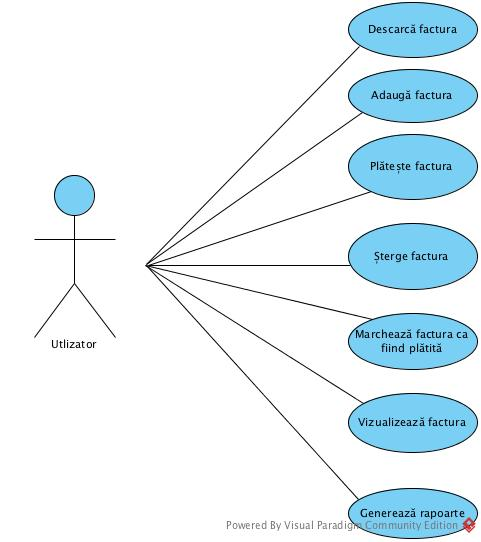
\includegraphics{UseCaseDiagram}
\end{center}

\section{Descrierea funcționalităților}

Baza de date aleasă este MySQL. Ea conține un tabel denumit "Factură" și la care este mapată, cu ajutorul adnotărilor (Hibernate), clasa Java cu numele de "Factură". Tabelul conține 9 câmpuri utilizate pentru stocarea facturilor. Câmpurile sunt:
\begin{addmargin}[4em]{1em}
	\begin{itemize}
		\item Id - stochează id-ul unei facturi și se autoincrementează de fiecare dată când se introduce o nouă factură în baza de date
		\item Utilitate - stochează tipul de utilitate al facturii respective (de exemplu: Telefonie, Gaze naturale, etc).
		\item Companie - stochează numele companiei pentru factura curentă (de exemplu: Orange, E-ON, etc).
		\item Data emiterii - stochează data în care s-a emis factura respectivă
		\item Data scadentă - stochează data la care factura respectivă devine scadentă ( data până la care se poate plăti factura, după această dată plata va fi posibilă dar se vor plăti și taxele de întârziere)
		\item Numărul facturii - stochează numărul facturii curente
		\item Status - stochează informația dacă o factură este plătită sau nu
		\item Total de plată - suma totală de plată pentru factura respectivă
		\item Link - reprezintă calea unde este stocată factura în calculator. Factura este stocată în calculator sub forma unui fișier de tip PDF
	\end{itemize}
\end{addmargin}

Tabelul a fost creat prin introducerea unei sintaxe de tip SQL. Sintaxa respectivă este:\\\\
CREATE TABLE 'Factura' (\\
'id' bigint(20) NOT NULL AUTO\_INCREMENT,\\
'UTILITATE' varchar(20) DEFAULT NULL,\\
`COMPANIE` varchar(255) DEFAULT NULL,\\
`DATA\_EMITERII` datetime DEFAULT NULL,\\
`DATA\_SCADENTA` datetime DEFAULT NULL,\\
`NR\_FACTURA` varchar(255) DEFAULT NULL,\\
`STATUS` varchar(255) DEFAULT NULL,\\
`TOTAL\_PLATA` float DEFAULT NULL,\\
`LINK` varchar(255) DEFAULT NULL,\\
PRIMARY KEY (`id`)\\
) ENGINE=InnoDB AUTO\_INCREMENT=55 DEFAULT CHARSET=latin1;\\

Fereastra principală este alcătuită dintr-un JFrame care înglobează mai multe elemente (JTable, JButton, JPanel, Font). Aceste elemente sunt declarate după cum urmează:
\begin{center}
	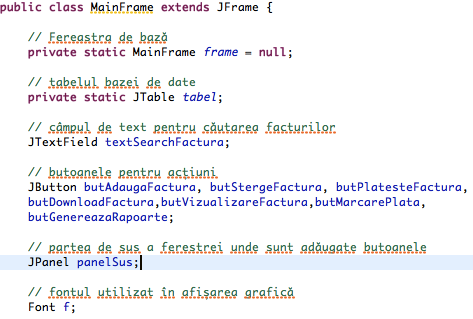
\includegraphics{FereastraPrincipala}
\end{center}

De asemenea, mai conține trei variabile de tip boolean care marchează tipul de acțiune selectat la apăsarea unui buton. Aceste variabile sunt definite după cum urmează și cu ajutorul lor se realizează operațiile de adăugare, descărcare și achitare a unei facturi.
Aceste variabile sunt definite după cum urmează:
\begin{figure}[h]
	\centering
	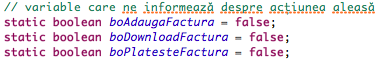
\includegraphics{VariabileAjutatoare}
	\caption{Variabilele ajutătoare}
\end{figure}

Atunci când aplicația rulează, practic rulează fereastra principală. De aici utilizatorul poate să aleagă ce să facă mai departe. Fereastra principală este redată în imaginea următoare:
\begin{center}
	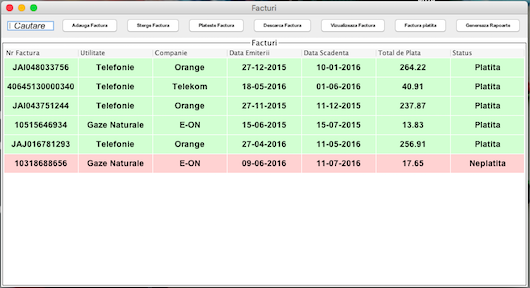
\includegraphics{FereastraPrincipalaVizualizare}
\end{center}

Butonului "Adauga Factura" îi este adăugat o acțiune de tipul ActionListener care se declanșează în momentul apăsării acestuia. ActionListener-ul va seta cu valoarea TRUE variabila "boAdaugaFactura" și va rula fereastra unde sunt afișate toate companiile.

Fereastra "Companii" (figura xx.xx) este alcătuită din 6 butoane, un buton pentru fiecare companie. Imaginile de fundal ale butoanelor sunt reprezentate de siglele companiilor. Fiecare companie are asociat un buton care la rândul lui are selectat ca și imagine de fundal sigla companiei respective. Fiecare buton are, de asemenea, mapat un ActionListener pentru tratarea evenimentului de apăsare a acestuia.  În momentul apăsării unui buton (alegerea unei companii) se verifică opțiunea selectată anterior, adică opțiunea de adăugare (variabila "boAdaugaFactura" are valoare TRUE) sau opțiunea de descărcare (variabila "boDescarcaFactura" are valoarea TRUE). Dacă opțiunea de adăugare a unei facturi este cea selectată, un element de tipul JFIleChooser (Figura xx.xx) va apărea pe ecran, acesta permițându-ne să alegem fișierul de tip PDF pe care vrem să îl introducem în baza de date. 
După ce vom selecta fișierul dorit și vom confirma selectarea acestuia, prin intermediul Apache PDFBox va începe procesul de extragere a textului din fișierul respectiv. Se crează o instanță de tip PDFParser care va primi ca paramentru calea către fișierul respectiv, după care va parcurge fișierul și îi va stoca tot conținutul de text într-o singură variabilă de tip String. După aceea se va împărți textul pe rânduri, pentru a fi mai ușor de extras datele necesare din el. \\\\
PDFTextStripper pdfStripper = null;\\
PDDocument pdDoc = null;\\
COSDocument cosDoc = null;\\
File file = new File(filePath);\\
PDFParser parser = new PDFParser(new FileInputStream(file));\\
parser.parse();\\
cosDoc = parser.getDocument();\\
pdfStripper = new PDFTextStripper();\\
pdDoc = new PDDocument(cosDoc);\\
pdfStripper.setStartPage(1);\\
pdfStripper.setEndPage(2);\\
String parsedText = pdfStripper.getText(pdDoc);\\
String lines[] = parsedText.split("\%\%r?\%\%n");\\

 După ce s-au extras datele necesare, se va crea o clasă de tip Factură (clasă ce este mapată prin Hibernate la baza de date) și se setează atributele acesteia cu valorile extrase din textul parcurs. După aceea se realizează conexiunea la baza de date prin intermediul unui obiect de tip EntityManager după care se introduce obiectul de tip Factura în baza de date:  \\\\
 Factura f=new Factura();\\
 f.setNrFactura(nr);\\
 f.setUtilitate(utilitate);\\
 f.setCompanie(companie);\\
 f.setDataEmiterii(date);\\
 f.setDataScadenta(date2);\\
 f.setTotalPlata(total);\\
 f.setStatus(status);\\
 f.setLink(link);\\
 String PERSISTENCE\_UNIT\_NAME = "persistenceIG";\\
 EntityManagerFactory factory;\\
 factory = Persistence.createEntityManagerFactory(PERSISTENCE\_UNIT\_NAME);\\
 EntityManager em = factory.createEntityManager();\\
 EntityTransaction et = em.getTransaction();\\
 et.begin();\\
 em.persist(f);\\
 et.commit();\\
 
 Un mesaj va apărea pe ecran și ne va informa unul din următoarele lucruri: factura este adăugată cu succes (Figura xx.xx), factura este deja existentă în baza de date (Figura xx.xx) sau că a apărut o eroare la extragerea textului din fișierul respectiv (Figura xx.xx). De obicei, acest lucru se întâmplă când a fost selectat fișierul greșit, care nu corespunde companiei alese. În cazul în care factura a fost introdusă cu succes în baza de date, fereastra principală se va reîmprospăta și noua factură introdusă putând fi văzută în tabelul bazei de date. În caz contrar, nu se va întâmpla nimic, utilizatorul putând să reia operația sau să aleagă alta.
\begin{figure}[!ht]
	\centering
	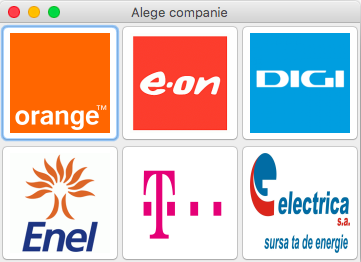
\includegraphics{Companii}
	\caption{Fereastra "Companii"}
\end{figure}

\begin{figure}[!ht]
	\centering
	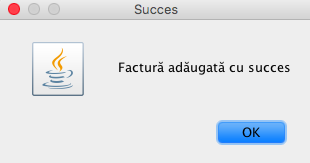
\includegraphics{FacturaAdaugataSucces}
	\caption{Mesajul transmis dacă factura este adăugată cu succes în baza de date}
\end{figure}

\begin{figure}[!ht]
	\centering
	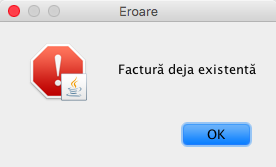
\includegraphics{FacturaExistenta}
	\caption{Mesajul transmis dacă factura este deja în baza de date}
\end{figure}

\begin{figure}[!ht]
	\centering
	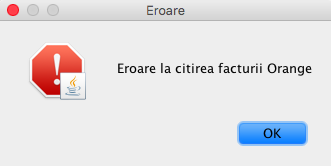
\includegraphics{EroareCitireaFacturii}
	\caption{Mesajul transmis dacă factura este adăugată cu succes în baza de date}
\end{figure}

\begin{figure}[!ht]
	\centering
	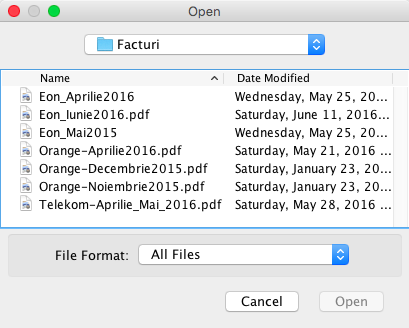
\includegraphics{FileChooser}
	\caption{Elementul de tip JFileChooser}
\end{figure}


Butonul "Sterge Factura" are, de asemenea, mapat un ActionListener pentru gestionarea evenimentelor. Prin simpla apăsare a butonului, acesta se declanșează. Primul pas este acela de a verifica dacă este selectată o singură factură, cu ajutorul funcției "getSelectedRows()" care returnează un tablou conținând indecșii rândurilor selectate din tabel. Dacă lungimea tabloului este 1, atunci este selectată o singură factură. În cazul în care nu este selectată o singură factură, un mesaj de atenționare va fi afișat pe ecran (Figura XX.XX). Dacă este selectată o singură factură, un mesaj de întrebare va apărea pe ecran în care utilizatorul va fi întrebat dacă este sigur că vrea să șteargă factura (Figura XX.XX). Dacă acesta răspunde afirmativ, se va realiza o conexiune la baza de date, se va stoca numărul facturii selectate și se va șterge factura cu acel număr din baza de date. Codul Java și SQL care face acest lucru este:
\\
Query query = em.createQuery("DELETE FROM Factura f WHERE f.nrFactura = :nrFact");\\
query.setParameter("nrFact", nrFactura);\\

Dacă utilizatorul se răzgândește și nu vrea să mai șteargă factura selectată, atunci nu se va întâmpla nimic, mesajul de întrebare va dispărea de pe ecran. Dacă factura este ștearsă cu succes, un mesaj de confirmare va fi afișat pe ecran (Figura XX.XX), după care se va reîmprospăta fereastra principală, factura ștearsă ne mai existând în baza de date. În caz contrar, un mesaj de eroare (Figura XX.XX) va înștiința utilizatorul cu privire la acest lucru.

\begin{figure}[!ht]
	\centering
	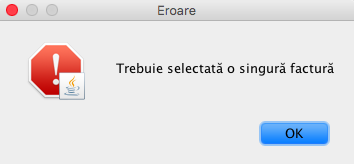
\includegraphics{TrebuieSelectata1Factura}
	\caption{Mesajul care informează utilizatorul că nu a selectat o singură factură}
\end{figure}

\begin{figure}[!ht]
	\centering
	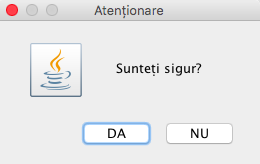
\includegraphics{SuntetiSigur}
	\caption{Mesaj de întrebare - utilizatorul este întrebat dacă este sigur de alegerea făcută}
\end{figure}

\begin{figure}[!ht]
	\centering
	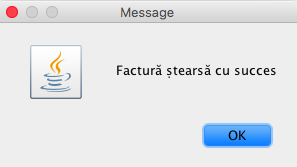
\includegraphics{FacturaStearsaSucces}
	\caption{Mesajul prin care utilizatorul este informat că factura a fost ștearsă cu succes}
\end{figure}

Atunci când butonul "Plateste Factura" este apăsat, se declanșează evenimentul produs de ActionListener-ul respectiv. Primul pas este acela de a verifica dacă este selectată o singură factură. În cazul în care nu este selectată, se va afișa un mesaj de eroare (Figura XX.XX) și se va încheia procesul de plată. Dacă este selectată o singură factură, se verifică dacă factura respectivă este plătită. Dacă aceasta este plătită, se va afișa un mesaj de eroare (Figura XX.XX). Dacă nu este plătită, se verifică dacă utilizatorul a introdus în trecut datele cardului necesare realizării plății (numărul, titularul, data expirării, codul de securitate). Aceste date sunt stocate într-un fișier din momentul introducerii acestora. Aplicația va căuta să vadă dacă acest fișier există. Dacă acest fișier nu există, va apărea o fereastră (Figura XX.XX) în care utilizatorului i se va cere să introducă datele cardului. După ce câmpurile au fost completate, prin apăsarea butonului "Introduceți datele" se declanșează ActionListener-ul butonului respectiv, care verifică dacă toate câmpurile au fost completate. Dacă datele sunt completate, se va crea un fișier în care se vor stoca datele extrase din câmpurile completate, fiecare informație va fi stocată pe un singur rând (Figura xx.xx). Dacă datele cardului au fost introduse la o plată anterioară, pasul de introducere a acestora în fișier va fi sărit. Următorul pas este acela de a intra în contul de abonat al companiei respective și de a plăti factura. Pentru a realiza acest lucru, avem nevoie de datele de logare ale utilizatorului. Acestea au fost deja stocate într-un fișier al aplicației atunci când s-a produs descărcarea facturii. O fereastră a browser-ului Firefox va porni și cu prin intermediul Selenium va parcuge pașii necesari pentru a plăti factura. Când se ajunge la introducerea datelor cardului, se extrag datele din fișierul creat la începutul procesului de plată sau anterior și se introduc în câmpurile respective. Procesul de plată se încheie prin afișarea unui mesaj în browser, de către compania respectivă, în care se specifică faptul că plata s-a realizat cu succes. În caz contrar, acest lucru va fi evidențiat tot printr-un mesaj în browser al companiei respective. Aplicația nu poate să verifice faptul că datele cardului au fost introduse corect sau chiar datele de logare în contul de utilizator al companiei respective sunt corecte. 

\begin{figure}[!ht]
	\centering
	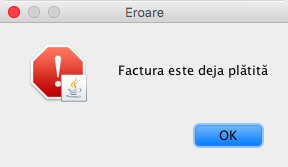
\includegraphics{FacturaPlatita}
	\caption{Mesajul prin care utilizatorul este informat că factura este deja plătită}
\end{figure}

\begin{figure}[!ht]
	\centering
	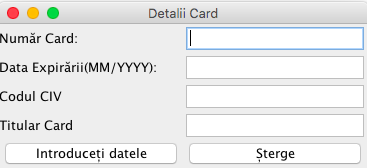
\includegraphics{DetaliiCard}
	\caption{Fereastra pentru adăugarea detaliilor despre cardul cu care se va realiza plata}
\end{figure}

\begin{figure}[!ht]
	\centering
	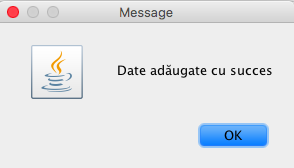
\includegraphics{DateCardSucces}
	\caption{Mesajul prin care utilizatorul este informat că datele cardului au fost stocate cu succes}
\end{figure}

\begin{figure}[!ht]
	\centering
	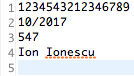
\includegraphics{DetaliiCardDocument}
	\caption{Modul în care sunt stocate datele cardului în fișier}
\end{figure}

După ce plata facturii a fost realizată cu succes, aceasta trebuie marcată ca fiind deja plătită. O factură, atunci când este introdusă în baza de date, este marcată ca fiind neachitată. Marcarea facturii ca fiind plătită se realizează prin apăsarea butonului "Factura platita". în momentul apăsării butonul intervine ActionListener-ul respectiv care gestionează acest eveniment. Primul pas este verificarea dacă o singură factură este selectată, în caz contrar se va afișa un mesaj de eroare (Figura XX.XX). Al doilea pas este verificarea dacă factura este neachitată, în caz contrar se va afișa un mesaj de eroare (Figura XX.XX). Dacă cele două verificări au fost trecute cu succes, se extrage din tabelul interfeței grafice numărul facturii selectate, se realizează o conexiune la baza de date și se actualizează statusul facturii care are numărul egal cu cel extras din tabelul interfeței grafice. Utilizatorul este înștiințat că operația s-a realizat cu succes printr-un mesaj (Figura XX.XX).

\begin{figure}[!ht]
	\centering
	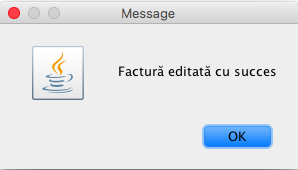
\includegraphics{EditareSucces}
	\caption{Mesajul prin care utilizatorul este informat că factura a fost marcată ca fiind plătită cu succes}
\end{figure}


\chapter{Concluzii}

\begin{thebibliography}{9}
	\bibitem{cursPracticJava}  Cristian Frăsinaru, {\em Curs Practic de Java}, Editura Maxitrom, 2005
	\bibitem{thinkJava}  Bruce Eckel, {\em Thinking in Java (Fourth Edition)}, Editura Pearson Education, 2006
	\bibitem{mySqlDeveloperLibrary} Paul DuBois, {\em MySQL Developer's Library (Forth edition)}, Editura Pearson Education, 2008
	\bibitem{BeginningHibernate} Joseph Ottinger, Dave Minter, Jeff Linwood, {\em Beginning Hibernate (Third edition)}, Editura Appres, 2014
	\bibitem{PDFBoxOfficial} Apache PDFBox Official Documentation
	\\\texttt{https://pdfbox.apache.org/index.html}
	\bibitem{swingBook} Matthew Robinson, Pavel Vorobiev, {\em Java Swing (Second Edition)}, Editura Manning Publications, 2003
\end{thebibliography}
	
\end{document}